\section[The Riemann-Stieltjes Integral]{\hyperlink{toc}{The Riemann-Stieltjes Integral}}

\subsection{Definition of the Integral}
\begin{definition}{Partition}{6.1}
    A partition of $[a, b] \subset \RR$ is a set $\set{x_0, x_1, \ldots, x_n}$ (for some $n \in \NN$) such that:
    \begin{align*}
        a = x_0 \leq x_1 \leq x_2 \leq \ldots \leq x_{n-1} \leq x_n = b
    \end{align*}
\end{definition}

\begin{figure}[htbp]
    \centering
    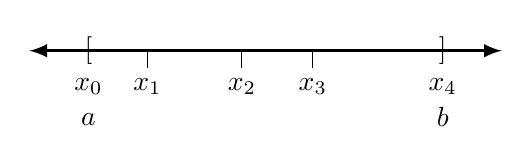
\begin{tikzpicture}[scale=1.5]
        \draw[very thick, latex-latex] (-2, 0) -- (2, 0);
        \node[] at (-1.5, 0) {$[$};
        \node[below] at (-1.5, -0.15) {$x_0$};
        \node[below] at (-1.5, -0.45) {$a$};
        \node[] at (1.5, 0) {$]$};
        \node[below] at (1.5, -0.15) {$x_4$};
        \node[below] at (1.5, -0.4) {$b$};
        \draw[] (-1, 0) -- (-1, -0.15);
        \node[below] at (-1, -0.15) {$x_1$};
        \draw[] (-0.2, 0) -- (-0.2, -0.15);
        \node[below] at (-0.2, -0.15) {$x_2$};
        \draw[] (0.4, 0) -- (0.4, -0.15);
        \node[below] at (0.4, -0.15) {$x_3$};
    \end{tikzpicture}
    \caption{Visualization of a partition $\set{x_0, x_1, x_2, x_3, x_4}$ of $[a, b]$. Note that the points in the partitions need not be equally spaced.}
    \label{fig27}
\end{figure}

\subsection{Criterion for Integrability}

\subsection{Properties of the Integral}

\subsection{Integration and Differentiation}

